\documentclass{article}
\usepackage{amsmath}
\usepackage{amssymb}
\usepackage{tikz}
\begin{document}

\section*{Exercício 12 - Seção 15.2}

\textbf{Enunciado:} Encontre a massa do sólido que é obtido ao encher a caixa $R=[0,1] \times [0,1] \times [0,2]$ com um material cuja densidade em cada ponto $(x,y,z)$ é dada por $\rho(x,y,z)=2xy+z$.

Solução:

A massa do sólido é dada por:

$$
m = \iiint_R \rho(x,y,z) \, dV.
$$

Usando coordenadas retangulares, temos:

\begin{align*}
m &= \int_{0}^{2} \int_{0}^{1} \int_{0}^{1} (2xy+z) \, dx \, dy \, dz \\
&= \int_{0}^{2} \int_{0}^{1} \left[ xy^2 + \frac{z}{2}x^2 \right]_{0}^{1} \, dy \, dz \\
&= \int_{0}^{2} \int_{0}^{1} \left( y^2 + \frac{z}{2} \right) \, dy \, dz \\
&= \int_{0}^{2} \left[ \frac{y^3}{3} + \frac{z}{2}y \right]_{0}^{1} \, dz \\
&= \int_{0}^{2} \left( \frac{1}{3} + \frac{z}{2} \right) \, dz \\
&= \left[ \frac{z}{3} + \frac{z^2}{4} \right]_{0}^{2} \\
&= \frac{11}{3}.
\end{align*}

Portanto, a massa do sólido é $\frac{11}{3}$.
\newpage

\section*{Exercício 36 - Seção 15.2}
\textbf{Enunciado:} Calcule a integral dupla $\iint_D x^2 , dA$, onde $D$ é a região delimitada pelos eixos coordenados e a reta $y=x/2$.

A região $D$ é um triângulo com vértices em $(0,0)$, $(2,1)$ e $(0,1)$, como mostra a figura abaixo:

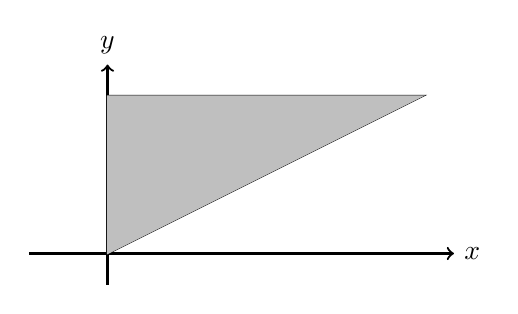
\begin{tikzpicture}[scale=2]

\draw[thick,->] (-0.5,0) -- (2.2,0) node[right] {$x$};
\draw[thick,->] (0,-0.2) -- (0,1.2) node[above] {$y$};
\draw[thick] (0,0) -- (2,1) node[midway, above left] {$y=x/2$} -- (0,1) -- cycle;
\filldraw[gray!50] (0,0) -- (2,1) -- (0,1) -- cycle;
\end{tikzpicture}

Podemos expressar $D$ como $D={(x,y),|,0\leq x\leq 2, 0\leq y\leq x/2}$.

Então, temos:

\begin{align*}
\iint_D x^2 , dA &= \int_0^2 \int_0^{x/2} x^2 , dy , dx \\
&= \int_0^2 x^2\cdot \left(\int_0^{x/2} dy\right) , dx \\
&= \int_0^2 x^2 \cdot \frac{x}{2} , dx \\
&= \frac{1}{2} \int_0^2 x^3 , dx \\
&= \frac{1}{2} \cdot \frac{x^4}{4} \Bigg|_0^2 \\
&= \frac{2^4}{2\cdot 4} \\
&= \boxed{2}.
\end{align*}

Portanto, a integral dupla $\iint_D x^2 , dA$ tem valor igual a $2$.

\newpage
\section*{Exercício 46 - Seção 15.2}
\textbf{Enunciado:} Esboce a regiao de integracao e mude a ordem de integracao.

Esboço da região de integração:

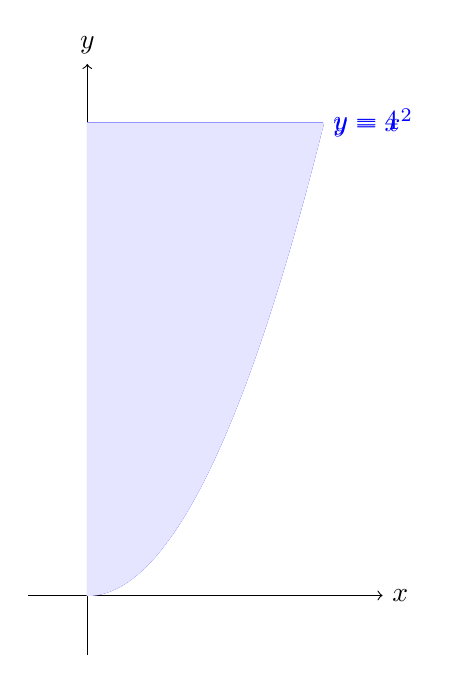
\begin{tikzpicture}[scale=1.5]
\draw[->] (0,-0.5) -- (0,4.5) node[above] {$y$};
\draw[->] (-0.5,0) -- (2.5,0) node[right] {$x$};
\draw[blue, domain=0:2, smooth, variable=\x] plot ({\x},{\x*\x}) node[right] {$y = x^2$};
\draw[blue, domain=0:2, smooth, variable=\x] plot ({\x},{4}) node[right] {$y=4$};
\filldraw[blue!10, domain=0:2, variable=\x, smooth, samples=100] plot ({\x},{\x*\x}) -- (2,4) -- (0,4) -- cycle;
\end{tikzpicture}

Mudança de ordem de integração:

$\int_0^2 \int_{x^2}^4 f(x, y) dydx = \int_0^4 \int_0^{\sqrt{y}} f(x, y) dxdy$

Esboço da nova região de integração:

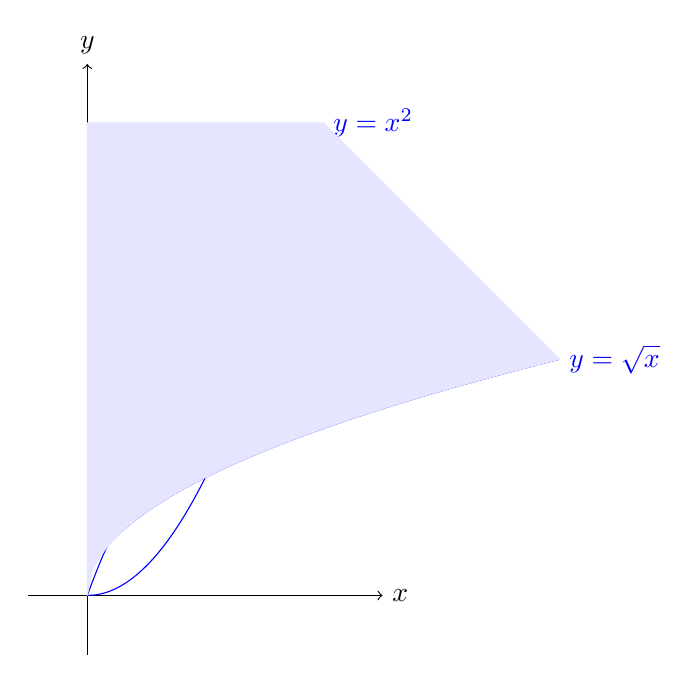
\begin{tikzpicture}[scale=1.5]
\draw[->] (0,-0.5) -- (0,4.5) node[above] {$y$};
\draw[->] (-0.5,0) -- (2.5,0) node[right] {$x$};
\draw[blue, domain=0:2, smooth, variable=\x] plot ({\x},{\x*\x}) node[right] {$y = x^2$};
\draw[blue, domain=0:4, smooth, variable=\x] plot ({\x},{sqrt(\x)}) node[right] {$y = \sqrt{x}$};
\filldraw[blue!10, domain=0:4, variable=\x, smooth, samples=100] plot ({\x},{sqrt(\x)}) -- (2,4) -- (0,4) -- cycle;
\end{tikzpicture}

\end{document}
